%\title{Wits Q poster}
\documentclass[a0,portrait]{a0poster}
\usepackage{a0size}
\usepackage{multicol} % This is so we can have multiple columns
    \columnsep=100pt % White space between the columns
    \columnseprule=3pt % Thickness of the black line between the columns
    
% \usepackage{pgfpages}
% \pgfpagesdeclarelayout{resize and center}
% {
%   \def\pgfpageoptionborder{0pt}
% }
% {
%   \pgfpagesphysicalpageoptions
%   {%
%     logical pages=1,%
%     physical height=\pgfpageoptionheight,%
%     physical width=\pgfpageoptionwidth%
%   }
%   \pgfpageslogicalpageoptions{1}
%   {%
%     resized width=\pgfphysicalwidth,%
%     resized height=\pgfphysicalheight,%
%     border shrink=\pgfpageoptionborder,%
%     center=\pgfpoint{.5215\pgfphysicalwidth}{.47\pgfphysicalheight}%
%   }%
% }
% \pgfpagesuselayout{resize and center}[a2paper,landscape]

\usepackage[super]{natbib}
\usepackage[svgnames]{xcolor} % Specify colors by their 'svgnames'
\usepackage{times} % Use the times font
\usepackage{graphicx}
    \graphicspath{{figures/}} % Location of the graphics files
\usepackage{booktabs} % Top and bottom rules for table
\usepackage[font=small,labelfont=bf]{caption}
\usepackage{amsfonts, amsmath, amsthm, amssymb}
\usepackage{wrapfig} % Allows wrapping text around tables and figures

\begin{document}
%----------------------------------------------------------------------------------------
%	POSTER HEADER 
%----------------------------------------------------------------------------------------
%Left Logo
\begin{minipage}[c]{0.08\linewidth}%

\includegraphics[width=\linewidth]{witslogo}\\%
\end{minipage}%
%Central
\begin{minipage}[c]{0.78\linewidth}%
\centering%
%Main Title
\veryHuge \color{NavyBlue} \textbf{How can Quantum Computing improve practical  Machine Learning today?}%
%Sub title
 \color{Black}\\[0.3cm]%
\Huge\textit{A suggestion on how near term quantum computing could be used to improve real life machine learning applications}\\[1.2cm]%
%Authors
\large \textbf{Tau Merand\textsuperscript{$\dagger$}}\\[0.5cm]%
%Institutes
\normalsize \textsuperscript{$\dagger$}School of Computer Science and Applied Mathematics, University of the Witwatersrand\\%
%Contacts
\texttt{tau.taylor.merand@gmail.com\\ github.com/TauMerand}\\%
\end{minipage}%
%Right Logo
\begin{minipage}[t]{0.12\linewidth}%

\includegraphics[width=\linewidth]{Wits-Q-logo.png}%
\end{minipage}%

\vspace{1.3cm}% Whitespace between the header and poster content

%----------------------------------------------------------------------------------------
% Body of Poster
\begin{multicols}{2} % This is how many columns your poster will be broken into, a portrait poster is generally split into 2 columns
%----------------------------------------------------------------------------------------
\color{Navy} % Navy color for the abstract
\section*{Abstract}
%\begin{abstract}
Quantum Computing (QC) has grown in leaps and bounds in the last 5-10 years; both in hardware and software .  Machine Learning (ML) is a field where large data-sets and massively parallel computing architectures have allowed for similar rapid improvements. We propose the use of current and near term QC as viable technology for boosting existing classical ML algorithms. However current QC hardware has drawbacks that makes QML on real life data infeasible, as such a hybrid approach using QML for model selection and Classical ML (CML) for actual learning from data and for inference is suggested. The exponential nature of super-positioned qubits can be leveraged to perform classically hard optimisations efficiently\cite{prezsalinas2019data}. However due to limitations in memory, qubit capacity and coherence times we think it is necessary to limit the use of QC to selecting effective model hyperparameters and then classically training the resultant model on large data. It is hopeful that this approach may yield better or faster learning due to the addition of QC while still being feasible to implement now or in the very near future. Good algorithmic results have been achieved by QCs on small state spaces so it seems promising to reframe hyperparameter selection as a QC problem and then execute a classical training-on-data gradient descent type algorithm on classical computing architectures. This approach seems likely to yield practical speed-ups or improvements in the ML sphere while QC hardware is still ill equipped to deal with real data sets\cite{mcclean2018barren}.
%\end{abstract}
%----------------------------------------------------------------------------------------
\color{DarkSlateGray}
\section*{QML for hyper-learning, CML for Learning  and Inference}
Applying ML to the real world generally revolves around training some model on data and then utilising that trained model for inference. Many factors affect the end efficacy of the model. Artificial Neural Networks (ANNs), in particular, are very sensitive to structure, namely: layers, size, activation functions and regularisation techniques. The selection of these generally follow current best practices but are not very well understood so producing an effective end model for an application is often more art than science\cite{zoph2016neural}. Following this drawback extensive work has been done in using optimisation methods for selecting these parameters; however the current best performing approaches use reinforcement learning for the creation of models\cite{zoph2016neural}. This is very computationally expensive since classical state exploration usually involves generating a model and training it to completion. We suggest that current QC has reached a stage where it can be used efficiently to perform this model selection for real world machine learning applications. The proposed method would roughly follow the procedure:
\begin{enumerate}\color{SaddleBrown}
	\item Use some QML algorithm, on small subsample of the training data, to optimise against some metric $f(\theta_{1...n})$, where $\theta_{1...n}$ would be the model hyperparameters such as depth, layers, activation functions etc. of the resultant CML model
	\item Train an CML with the selected parameters on the entire dataset as per the CML algorithm.
	\item Update the QML model using an overall cost function, $g(\theta_{1...n}, \phi_{1...n}, E(\theta_{1...n}) )$ where $\phi_{1...n}$ are the internal parameters of the QML model and $E(\theta_{1...n})$ is the cost function of the CML mode.
	\item Repeat as many times as feasible, until a required accuracy or metric is reached or until the QML algorithm converges.
\end{enumerate}
\color{DarkSlateGrey}
This approach is based on the ability to work with qubits in superposition allowing for search of the model parameter state space to be much more efficient than classical approaches while trying to mitigate the current drawbacks of QC and ultimately producing a model that can be used practically for inference. At this time QC has definitely not proliferated enough for companies to use QC cloud offerings for inference\cite{national2019quantum}. This approach hopes to reduce overall training times while still producing models that are effectively structured with best possible loss. The possible strength of this approach is based on how well QC does at state space search in superposition\cite{prezsalinas2019data} as opposed to something like reinforcement learning where exploration has to take place one state at a time\cite{zoph2016neural}. Finally this approach tries to take into account the "qubit capacity" of current QC's. While the number of qubits doesn't determine a bound on computational power in the same way as a classical computers' bits do\cite{prezsalinas2019data}, current QC are definitely at the start of the Quantum Moore's Law curve shown in figure \ref{graph}, so limiting the number of parameters to optimise is of benefit at this time.
%----------------------------------------------------------------------------------------
\begin{center}\vspace{1cm}
	\begin{tabular}{l c c c c}
		\toprule
		& \shortstack{Tenerife	\\ (IBM Q Experience)}
		& \shortstack{Tokyo\\ 	(IBM Q Network) }
		& \shortstack{Poughkeepsie\\	(IBM Q Network) }
		& \shortstack{IBM Q	 \\System One } \\
		\midrule
		\shortstack{Relaxation (T1) ($\mu s$)\\
			mean\\
			best\\
			worst}
		& \shortstack{51.1\\
			57.7\\
			42.3}
		& \shortstack{84.3\\
			148.5\\
			42.2}
		& \shortstack{73.2\\
			123.3\\
			39.4}
		& \shortstack{73.9\\
			132.9\\
			38.2}
		\\ 
		\midrule
		\shortstack{Dephasing (T2) ($\mu s$)\\
			mean\\
			best\\
			worst}
		&\shortstack{25.9\\
			40.2\\
			10.6}
		& \shortstack{49.6\\
			78.4\\
			24.3 }
		& \shortstack{66.2\\
			123.6\\
			10.8 }
		& \shortstack{69.1\\
			100.8\\
			39.2}
		\\ 
		\midrule
		\shortstack{Two-qubit error rates \\ ($\times 10^{-2}$)\\
			mean\\
			best\\
			worst}
		& \shortstack{4.02\\
			2.24\\
			5.76 }
		& \shortstack{2.84\\
			1.47\\
			7.12 }
		& \shortstack{2.25\\
			1.11\\
			6.61 }
		& \shortstack{1.69\\
			0.97\\
			2.85 }
		\\ 
		\midrule
		\shortstack{Single-qubit error rates  \\ ($\times 10^{-3}$)\\
			mean\\
			best\\
			worst}
		& \shortstack{1.65\\
			0.69\\
			3.44 }
		& \shortstack{1.99\\
			0.64\\
			6.09 }
		& \shortstack{1.07\\
			0.52\\
			2.77 }
		& \shortstack{0.41\\
			0.19\\
			0.82 }
		\\ 
		\bottomrule
	\end{tabular}
	\captionof{table}{\color{Green} Comparison of fundamental metrics of the quantum devices in four recent IBM Q systems\cite{IBM_2019}, showing the main issues current QC hardware has: T1 and T2 are too low for iterative QML on large data sets and errors are too high for accurate inference}\label{errortable}
\end{center}
\section*{Why not just do QML?}
  QC has seen significant successful research in creating QML algorithms. These algorithms usually fall into two general categories: those that mimic classical algorithms executed on a QC or those that utilise parametrized quantum circuits\cite{prezsalinas2019data}. The latter category shows significant promise for implementation on current and near term Noisy Intermediate Scale Quantum (NISQ) computers\cite{national2019quantum}, with massive performance gains while the former, while fascinating doesn't tend to result in the same gains.  However, as the name suggests NISQ machines are noisy and prone to error. In particular QCs are currently limited by qubit errors and coherence times; i.e the time it takes for information to "leak out" of the system\cite{IBM_2019}. As can be seen in table \ref{errortable} a QC only has tens to hundreds of microseconds before qubit states are lost and errors are still high when considering the sheer number of gate operations needed for complex tasks such as ML. This is not a hardware situation that is amenable to processing the large datasets that real world problems entail. Most speed-ups of QML over classical ML (CML) have been on small, proof-of-concept type examples; often run on simulators to reduce error. Another issue with QML is simply data input. While some exceptional techniques have been proposed and implemented for reading classical data onto qubits, they currently lack the speed or accuracy needed to actually be practical\cite{prezsalinas2019data}. The act of reading in gigabytes of data would probably take longer than the coherence of the system. 

%----------------------------------------------------------------------------------------
\section*{Looking to the Future}
Current QC definitely has its difficulties, in particular related to qubit error and short coherence times. The holy grail of this work will probably be error correcting qubit architectures, which will alleviate many of the current difficulties\cite{national2019quantum}.. With respect to this proposed protocol of restricting QML to hyper-learning - as QCs improve it will definitely become more feasible to move more of the learning into QCs however it seems plausible that inference may remain in the realm of classical computers for the foreseeable future. As shown in figure \ref{graph} IBM is forecasting growth in Quantum Volume in a similar manner to Moore's Law. If this continues to be accurate we will certainly be seeing QCs capable of practical computational tasks that are classically intractable in the near future, however until questions about memory and data transfer into a QC are answered those tasks may continue to lie in numerical optimisations rather than data based QML for a much longer time\cite{national2019quantum}.

\begin{minipage}[c]{0.45\linewidth}\vspace{0.5cm}%
	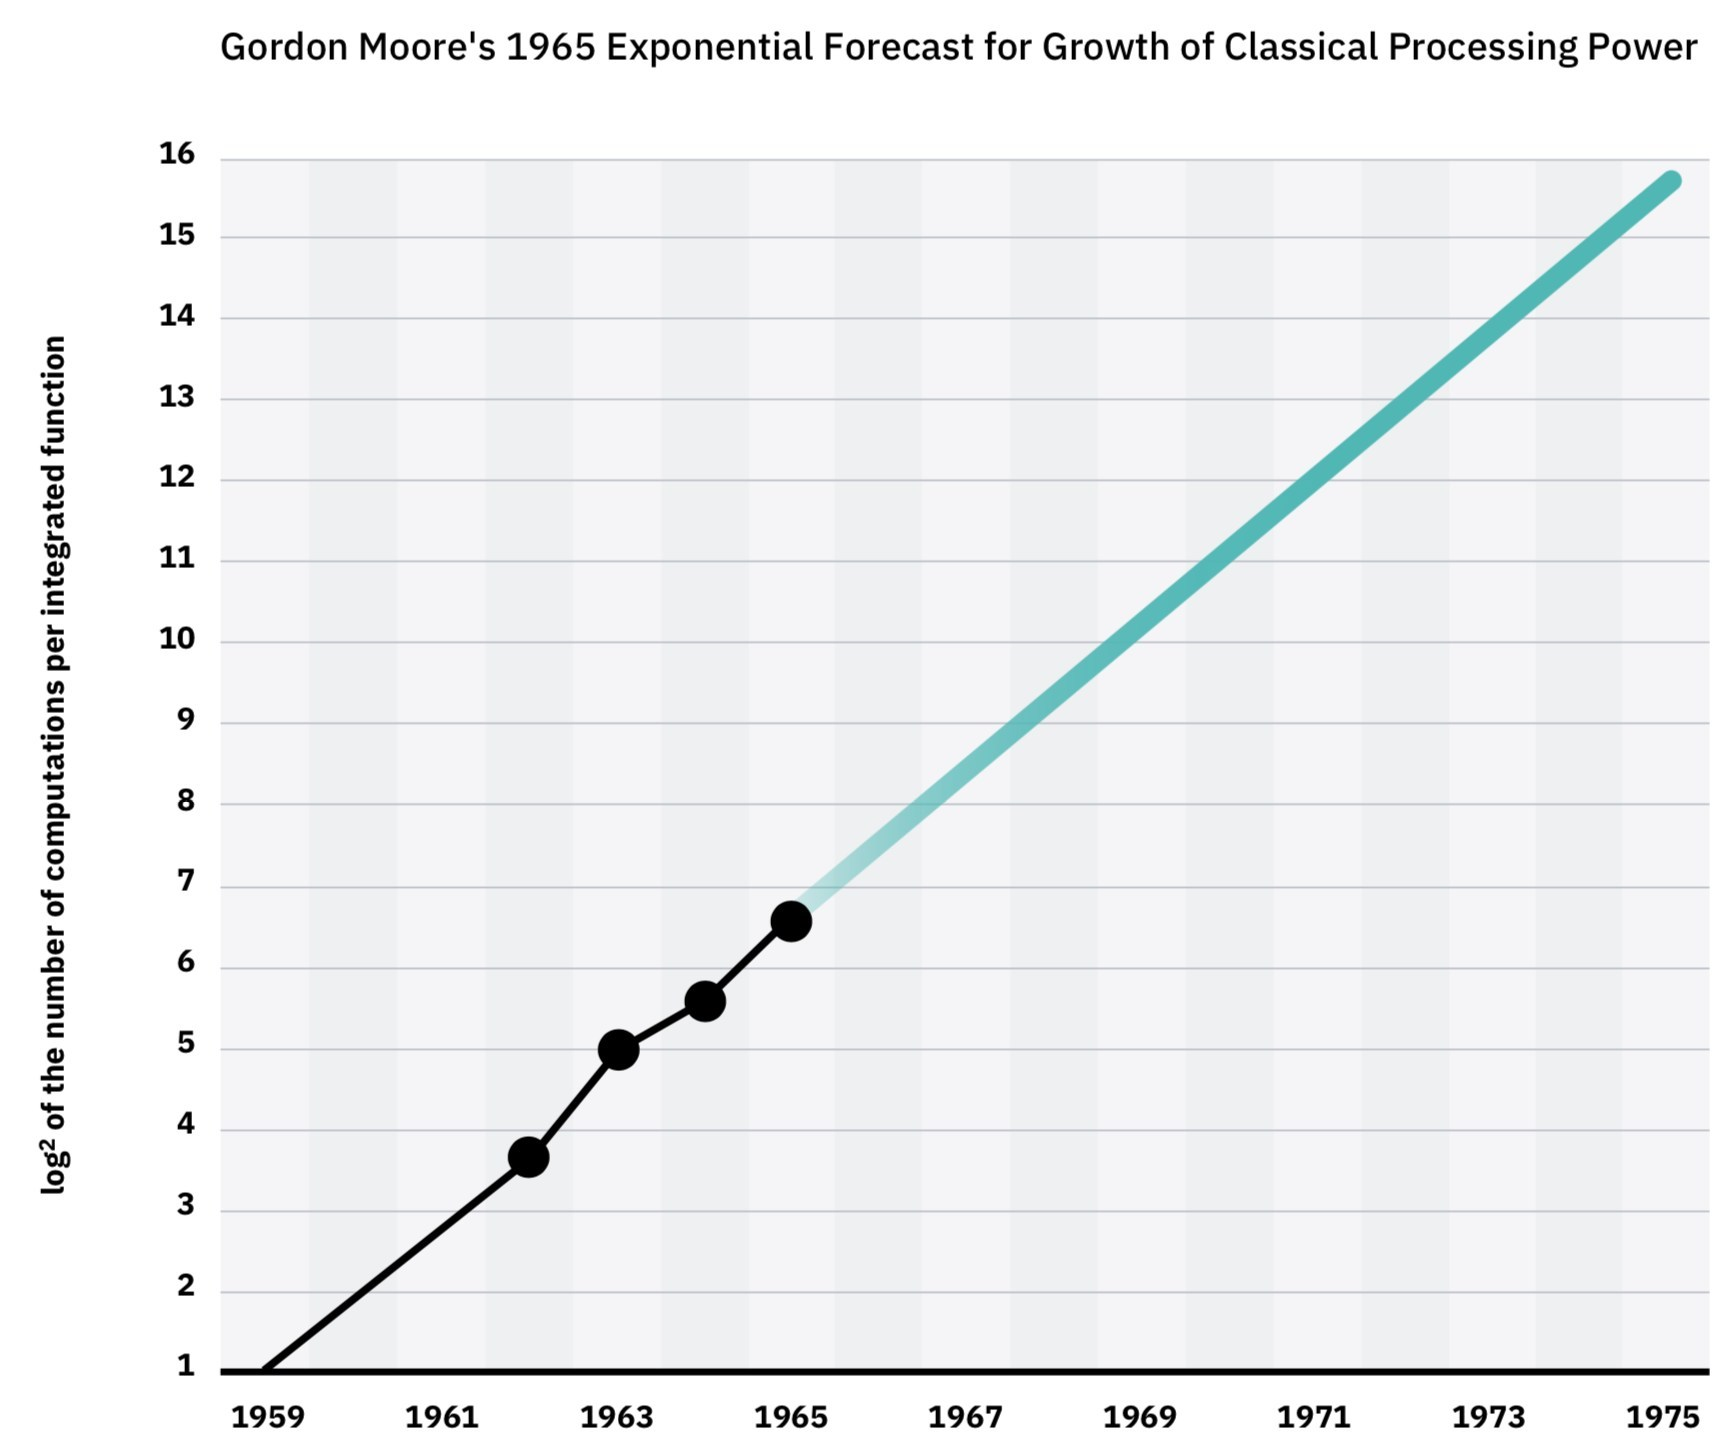
\includegraphics[width=\linewidth]{MooresLaw}\\%
\end{minipage}%
\begin{minipage}[c]{0.45\linewidth}%
	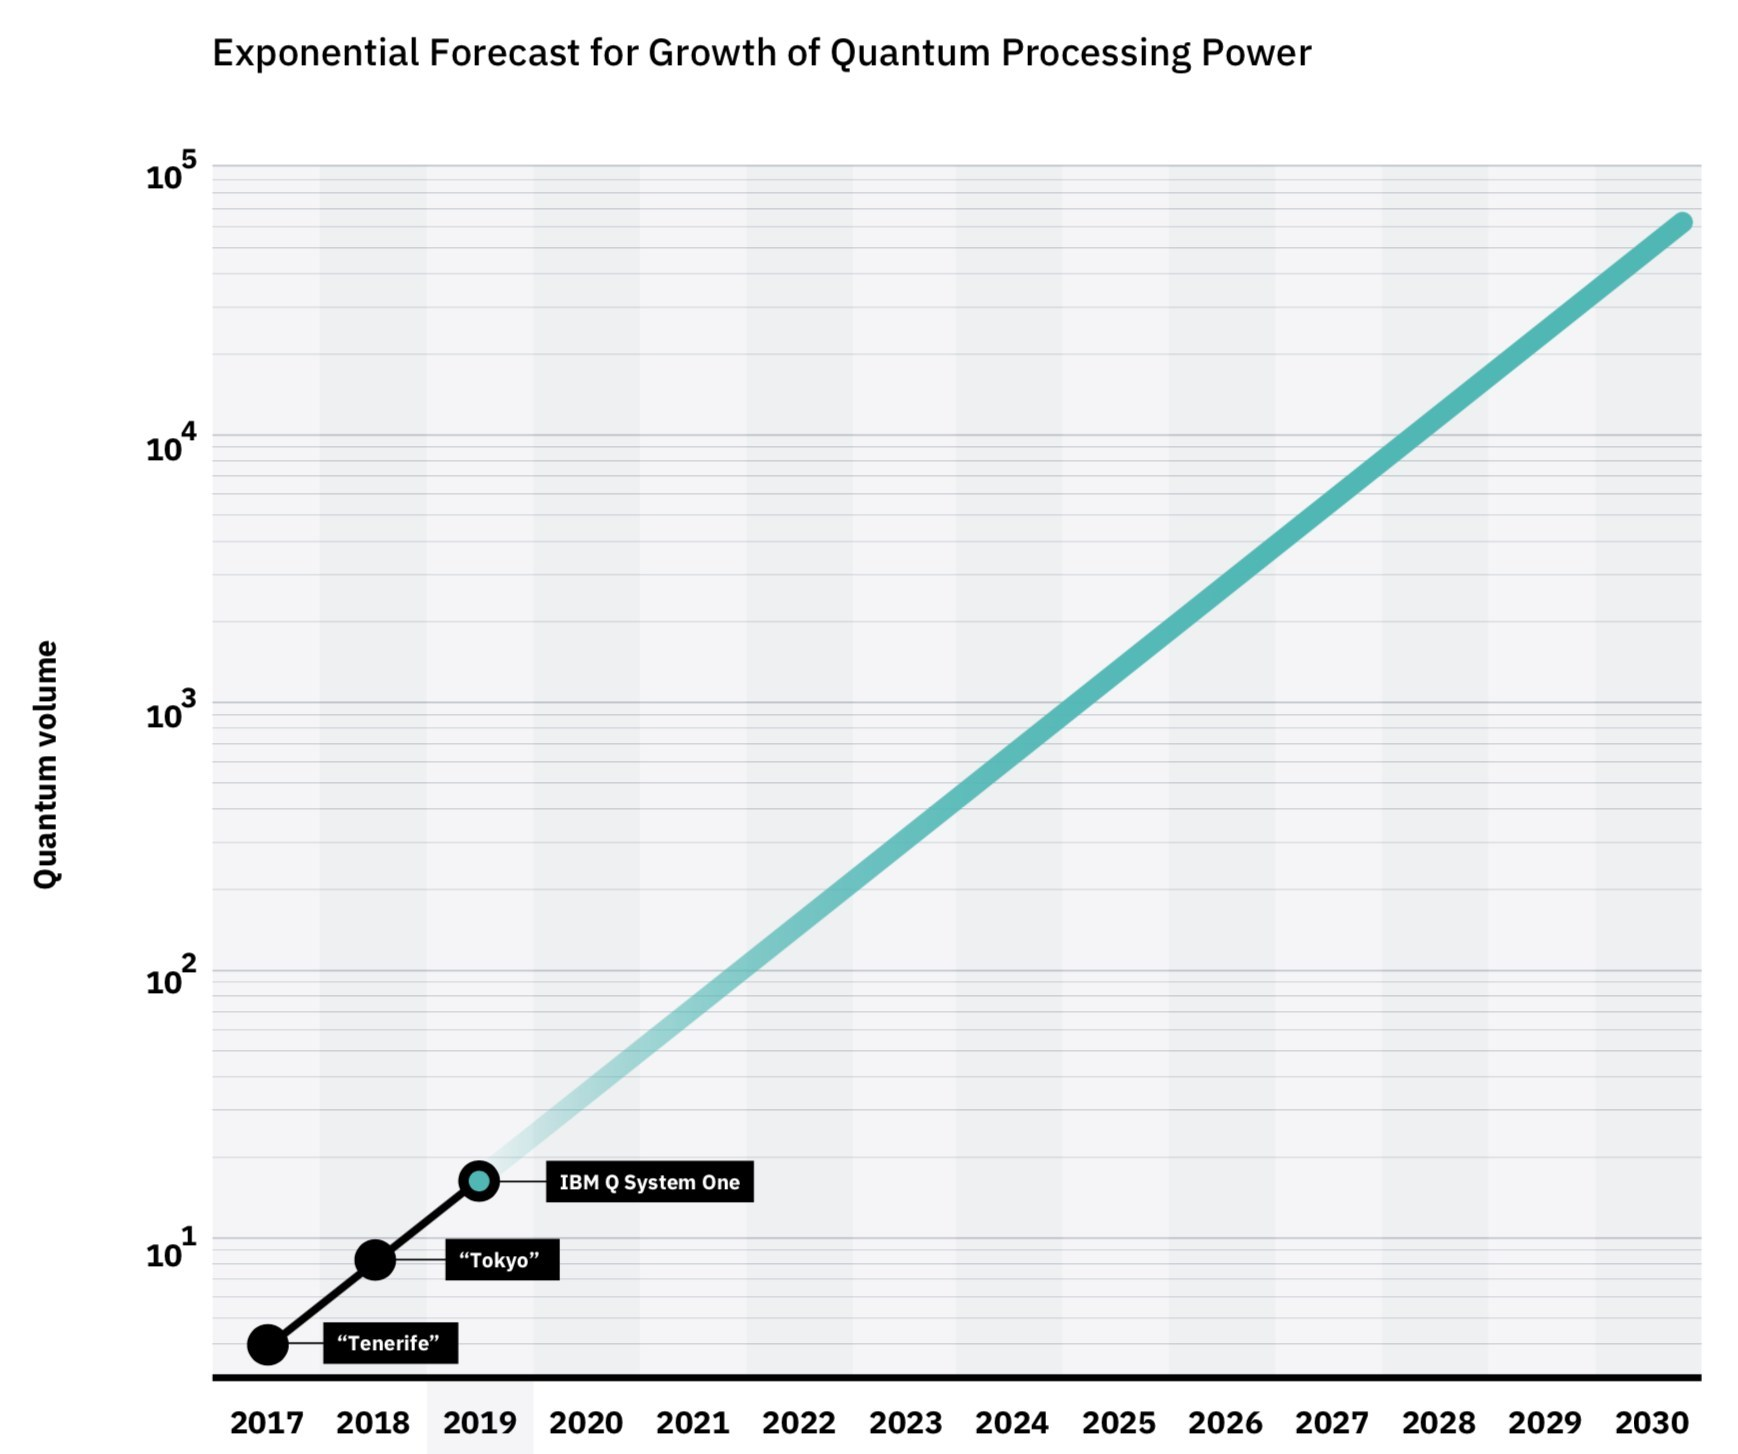
\includegraphics[width=\linewidth]{Qvolume}\\%
\end{minipage}%
\captionof{figure}{\color{Green}Moores's Law for classical architectures vs IBM's goal for Quantum Volume\cite{IBM_2019}, showing how bright the future looks with respect to QC but also that we are quite near the start of rapid QC growth. Practical Quantum only ML may still be decades away or may be just around the corner.}\label{graph}
%----------------------------------------------------------------------------------------
\color{SaddleBrown} % SaddleBrown color for the conclusions to make them stand out
\section*{Conclusions}
QC and QML have a lot of promise, but are currently issues with coherence times, errors and data input make QCs impractical for use for applied ML on large real life datasets. We proposed a method to allow for the use of QML in conjunction with CML in order to leverage the speed ups QC can offer to improve practical ML. In the future QML may become more practically applicable to ML but many large improvements will need to be made. The approach suggested here may allow QC to boost current applied CML algorithms with current and near term QC hardware. By limiting the QML portion to selecting (few) model parameters by optimising on a small data subset; issues around coherence times are hopefully mitigated while CML with those model parameters may allow for highly effective model structures to be selected for the specific applications in question without having to pay the computational cost of current classical approaches.
%----------------------------------------------------------------------------------------
\color{DarkSlateGray} % Set the color back to DarkSlateGray for the rest of the content
\section*{Further Research}
Obviously this does not offer any data to back up the claim that this is a viable approach to utilising QC for applied ML. Further research needs to be done by empirically comparing current best performing approaches to this method. Comparisons will need to compare across many axis such as training and test accuracy, generalisation error, iterations vs accuracy, iteration time etc. Research along a more mathematical approach to show that the composite loss function $g(\theta_{1...n}, \phi_{1...n}, E(\theta_{1...n}) )$ proposed would allow convergence with different QML and CML techniques is would also be interesting.
 %----------------------------------------------------------------------------------------
%\nocite{*} % Print all references regardless of whether they were cited in the poster or not
\bibliographystyle{plain} % Plain referencing style
\bibliography{biblio} % Use the example bibliography file sample.bib
%----------------------------------------------------------------------------------------
\section*{Acknowledgements}
Many thanks to the organisers of the WitsQ Quantum Computing Summer School as well as IBM. We have all learnt an incredible amount about an incredibly fascinating topic that would have been exceedingly difficult to learn by self study. 
%----------------------------------------------------------------------------------------
\end{multicols}
\end{document}